\documentclass[11pt,a4paper]{article}
\usepackage[utf8]{inputenc}
\usepackage[T1]{fontenc}
\usepackage[italian]{babel}
\usepackage{geometry}
\geometry{top=2.2cm,bottom=2.2cm,left=2.2cm,right=2.2cm}
\usepackage{graphicx}
\usepackage{xcolor}
\usepackage{amsmath, amssymb}
\usepackage{eurosym}
\usepackage{tcolorbox}
\tcbuselibrary{skins,breakable}
\usepackage{hyperref}
\usepackage{fancyhdr}
\usepackage{titlesec}
\usepackage{enumitem}
\usepackage{booktabs}
\usepackage{microtype}
\usepackage{tabularx}

% --- Palette Colori SIMO Macaron ---
\definecolor{simoPink}{HTML}{E24B6A}
\definecolor{simoDarkPink}{HTML}{B82D4B}
\definecolor{simoGreen}{HTML}{5CB87A}
\definecolor{simoDarkGreen}{HTML}{2D6A40}
\definecolor{simoCream}{HTML}{FFF5F7}
\definecolor{simoBorder}{HTML}{F8D3DC}
\definecolor{simoText}{HTML}{2E2325}
\definecolor{simoSubtle}{HTML}{6E5D61}
\definecolor{simoYellow}{HTML}{FFA000}
\definecolor{badgeBg}{HTML}{FDE8ED}

% --- Stile Hyperref ---
\hypersetup{
    colorlinks=true,
    linkcolor=simoDarkPink,
    urlcolor=simoPink,
    citecolor=simoDarkGreen
}

% --- Stile Testate e Pi\`e di Pagina ---
\pagestyle{fancy}
\fancyhf{}
\fancyhead[L]{\small\textbf{\color{simoPink}SIMO 2.0} \textendash{} Manuale d'Istruzioni per l'Utente}
\fancyhead[R]{\small\color{simoSubtle}\nouppercase{\leftmark}}
\fancyfoot[C]{\thepage}
\renewcommand{\headrulewidth}{0.4pt}
\renewcommand{\headrule}{\color{simoBorder}\hrule width\headwidth height\headrulewidth \vskip-\headrulewidth}

% --- Stile Titoli di Sezione ---
\titleformat{\section}
  {\normalfont\Large\bfseries\color{simoDarkPink}}{\thesection}{1em}{}[\color{simoBorder}\titlerule]
\titleformat{\subsection}
  {\normalfont\large\bfseries\color{simoText}}{\thesubsection}{1em}{}
\titleformat{\subsubsection}
  {\normalfont\normalsize\bfseries\color{simoDarkPink}}{\thesubsubsection}{1em}{}

% --- Box Grafici per Suggerimenti e Passaggi ---
\newtcolorbox{simobox}[2][]{
    enhanced,
    colback=simoCream,
    colframe=simoPink,
    coltitle=white,
    fonttitle=\bfseries,
    title=#2,
    arc=4mm,
    boxrule=1pt,
    left=4mm, right=4mm, top=3mm, bottom=3mm,
    drop shadow=black!10,
    #1
}

\newtcolorbox{tipbox}[1][Consiglio Pratico]{
    enhanced,
    colback=simoGreen!8,
    colframe=simoDarkGreen,
    coltitle=white,
    fonttitle=\bfseries,
    title=#1,
    arc=3mm,
    boxrule=0.8pt,
    left=3mm, right=3mm, top=2mm, bottom=2mm
}

\newtcolorbox{warnbox}[1][Attenzione]{
    enhanced,
    colback=simoYellow!10,
    colframe=simoYellow!90!black,
    coltitle=white,
    fonttitle=\bfseries,
    title=#1,
    arc=3mm,
    boxrule=0.8pt,
    left=3mm, right=3mm, top=2mm, bottom=2mm
}

\newcommand{\badge}[1]{%
  \colorbox{badgeBg}{\color{simoDarkPink}\small\textbf{#1}}%
}

\begin{document}

% ==============================================================================
% COPERTINA
% ==============================================================================
\begin{titlepage}
    \centering
    \vspace*{1.2cm}
    
    {\Huge \bfseries \color{simoPink} SIMO 2.0}\\[0.3cm]
    {\large \bfseries \color{simoDarkPink} Scalable Ingredient Management Organizer}\\[0.8cm]
    
    {\color{simoBorder}\rule{0.75\textwidth}{1.5pt}}\\[1.0cm]
    
    {\LARGE \bfseries \color{simoText} Manuale d'Istruzioni e Guida all'Uso}\\[0.4cm]
    {\normalsize \color{simoSubtle} Il tuo assistente intelligente per il ricalcolo delle dosi, la resa in cottura,\\
    i valori nutrizionali UE, il food cost al centesimo, la spesa e la cottura guidata}\\[1.5cm]
    
    \begin{tcolorbox}[
        enhanced,
        colback=white,
        colframe=simoPink,
        arc=6mm,
        width=0.82\textwidth,
        halign=center,
        boxrule=1.5pt,
        drop shadow=simoPink!20
    ]
        \vspace{0.3cm}
        \textbf{\color{simoDarkPink} Versione Software:} 2.0 (Release Ufficiale)\\[0.2cm]
        \textbf{\color{simoText} Piattaforma:} Sistema Operativo Android 8.0+ (Smartphone \& Tablet)\\[0.2cm]
        \textbf{\color{simoSubtle} Intelligenza Artificiale:} Dual Engine Google Gemini \& OpenAI ChatGPT\\[0.2cm]
        \textbf{\color{simoSubtle} Design System:} Soft Macaron Palette \& Bubble Typography\\[0.3cm]
    \end{tcolorbox}
    
    \vfill
    
    {\small \color{simoSubtle} Guida illustrata passo-passo per cuochi, pasticceri, panificatori, appassionati e professionisti\\
    \today}
    \vspace*{0.8cm}
\end{titlepage}

% ==============================================================================
% SOMMARIO
% ==============================================================================
\tableofcontents
\newpage

% ==============================================================================
% SEZIONE 1: INTRODUZIONE
% ==============================================================================
\section{Benvenuti in SIMO 2.0}

\textbf{SIMO} (\textit{Scalable Ingredient Management Organizer}) nasce per rispondere in modo scientifico, elegante ed intuitivo a un'esigenza fondamentale di chiunque operi in cucina, in pasticceria o in un laboratorio artigianale: \textbf{il calcolo proporzionale e analitico delle dosi, delle rese e dei costi}.

Spesso i ricettari tradizionali presentano formulazioni calibrate su dosi fisse (ad esempio una torta per 8 persone o un impasto per 500\,g di farina), ma le reali esigenze produttive sono mutevoli: un banchetto con 45 invitati, una fornitura di 80 cornetti, oppure una dispensa in cui sono rimasti solo 130\,g di burro o 2 uova. Inoltre, la moderna legislazione alimentare europea (Regolamento UE 1169/2011) impone una trasparenza rigorosa sia sugli \textbf{allergeni} sia sulla \textbf{dichiarazione nutrizionale} obbligatoria dei prodotti finiti.

\begin{simobox}{Le Caratteristiche e Innovazioni di SIMO 2.0}
SIMO non \`e un semplice taccuino di appunti, bens\`i un sofisticato \textbf{motore matematico e relazionale a grafo (DAG)}:
\begin{itemize}[leftmargin=*,noitemsep]
    \item \textbf{Ricalcolo Dinamico Diretto (Scaling):} Modifichi la resa (es. porzioni, pezzi, grammi) e tutti gli ingredienti si aggiornano istantaneamente con precisione decimale.
    \item \textbf{Modificatore Peso e Resa in Cottura:} Imposti la variazione di peso subita durante la cottura (calo peso negativo per evaporazione nel forno come per torte e carni, oppure aumento di massa positivo per assorbimento d'acqua come per pasta e riso).
    \item \textbf{Dichiarazione Nutrizionale UE Integrata (Reg. UE 1169/2011):} Tabella nutrizionale completa con i 6 valori fondamentali (Calorie, Carboidrati, Grassi, Proteine, Acqua, Sodio e Sale equivalente calcolato), espressi sia per 100\,g sia per singola porzione di prodotto finito cotto.
    \item \textbf{Reverse Scaling dalla Dispensa:} Inserisci la quantit\`a dell'ingrediente limitante rimasto in magazzino e SIMO riparametra l'intera ricetta a ritroso.
    \item \textbf{Sotto-Ricette Gerarchiche a Cascata (DAG):} Colleghi preparazioni base (es. \textit{Crema Pasticcera}) all'interno di ricette composte (es. \textit{Cornetto alla Crema}). La scalatura e gli allergeni si propagano automaticamente lungo l'intero albero matematico.
    \item \textbf{Food Cost al Centesimo ed Equivalenza Culinaria:} Calcolo in tempo reale del costo totale dell'impasto e del costo industriale per singola porzione, con conversioni metriche automatiche ($g \leftrightarrow kg$, $ml \leftrightarrow l$) ed equivalenza culinaria massa-volume 1:1.
    \item \textbf{Esportazione PDF Professionale A4 (Minimo 2 Pagine):} Genera schede tecniche vettoriali di laboratorio: Pagina 1 con metadati, ingredienti, food cost, allergeni e tabella nutrizionale UE; Pagina 2 con il procedimento di preparazione ad alta visibilit\`a in nero pieno.
    \item \textbf{Cooking Mode Protetta:} Schermo sempre attivo (\textit{Keep Screen On}) e timer multipli concorrenti con estrazione automatica dei tempi dalle istruzioni.
    \item \textbf{Assistente Chef AI Bivalente (Gemini \& ChatGPT):} Generazione completa, completamento intelligente delle dosi mancanti e stima nutrizionale non-distruttiva, con preservazione dell'unit\`a di misura desiderata (es. \textit{torta}, \textit{bicchieri}, \textit{panini}).
    \item \textbf{Nuova Categoria Predefinita Panini:} Categoria gastronomica dedicata per la panificazione e la paninoteca artigianale.
\end{itemize}
\end{simobox}

\newpage

% ==============================================================================
% SEZIONE 2: ESPLORARE IL RICETTARIO E LA SCHERMATA HOME
% ==============================================================================
\section{Esplorare il Ricettario e la Schermata Home}

All'avvio dell'applicazione verrai accolto dalla schermata principale (Figura~\ref{fig:home}), disegnata secondo una palette di colori pastello morbidi (\textit{Soft Macaron}) che garantisce un contrasto ideale sia alla luce naturale del laboratorio sia in ambienti di cottura. Grazie al motore di pre-caricamento asincrono immediato, l'intero ricettario viene popolato istantaneamente, eliminando qualsiasi schermata bianca transitoria.

\begin{figure}[h!]
    \centering
    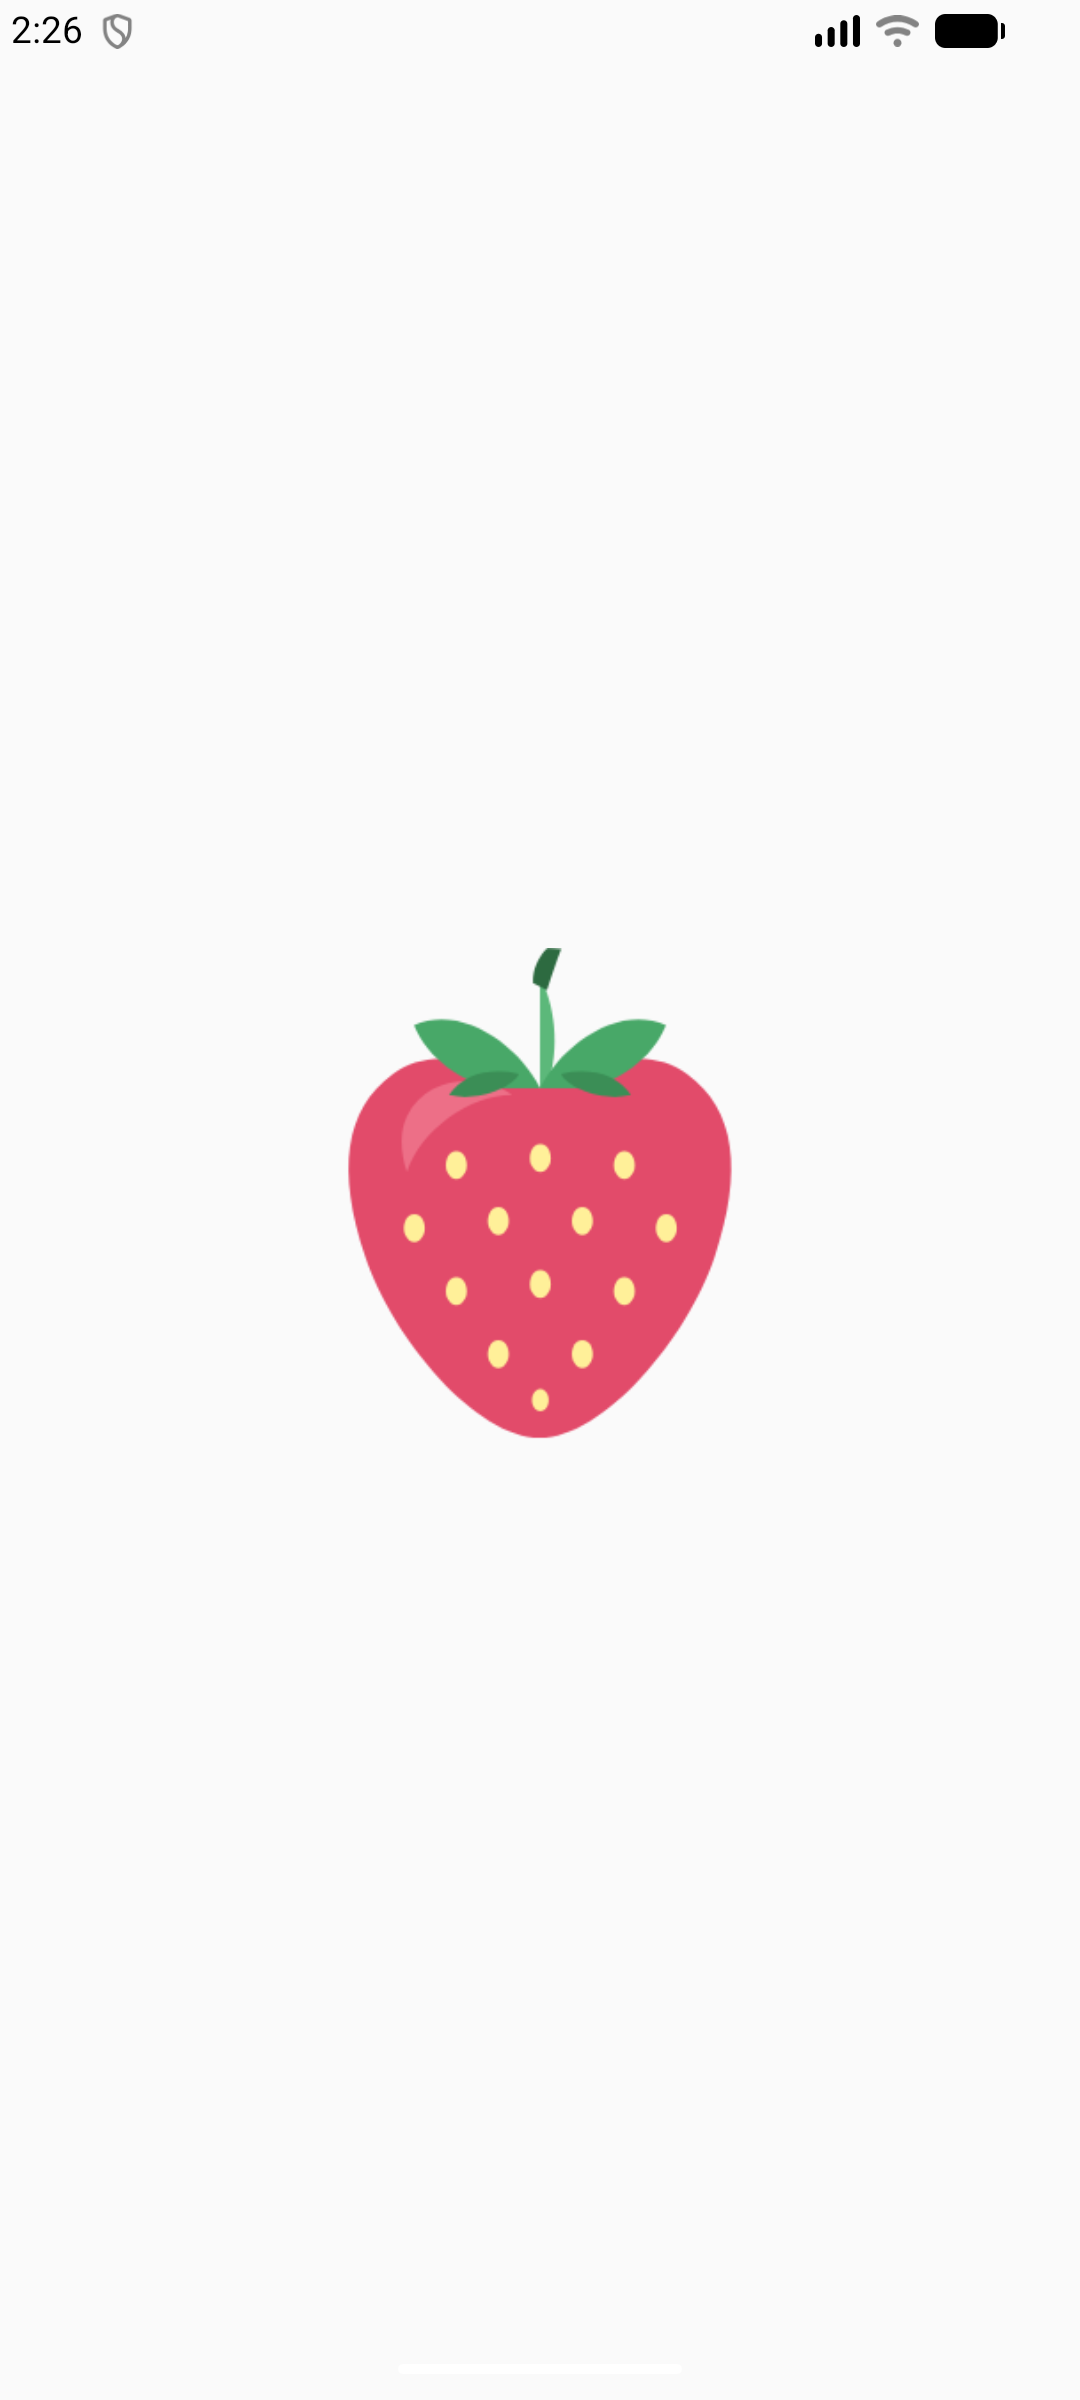
\includegraphics[width=0.48\textwidth]{images/screen_optimized_home.png}
    \caption{Schermata Principale di SIMO 2.0: elenco delle ricette con badge di categoria, resa base, calo cottura e barra di navigazione superiore.}
    \label{fig:home}
\end{figure}

\subsection{Comprendere la Scheda di ciascuna Ricetta}
Ogni elemento del ricettario mostra a colpo d'occhio i dati fondamentali:
\begin{itemize}[leftmargin=*]
    \item \textbf{Nome e Descrizione Culinaria:} Il titolo della ricetta e un breve riassunto delle sue caratteristiche organolettiche e procedurali.
    \item \textbf{Badge Categoria (\badge{Dolci}, \badge{Pizze}, \badge{Panini}, \badge{Primi}):} Segnala la tipologia di preparazione e permette il filtraggio tematico con un tocco.
    \item \textbf{Badge Resa Base:} Indica le dosi originali registrate (ad esempio \textit{Resa base: 8 porzioni}, \textit{10 cornetti} oppure \textit{500\,g}).
    \item \textbf{Icona Preferiti (Stella):} Con un semplice tocco sulla stella puoi contrassegnare o rimuovere qualsiasi ricetta dai tuoi preferiti.
    \item \textbf{Pulsanti Rapidi:} L'icona \textbf{Matita} apre la modifica della ricetta, il \textbf{Cestino} consente l'eliminazione sicura (con salvaguardia delle ricette correlate) e il pulsante \textbf{Vedi Ricetta} conduce direttamente alla console di dettaglio e ricalcolo.
\end{itemize}

\subsection{Ricerca, Categorie Predefinite e Ordinamento}
Nella barra superiore (\textit{Top Bar}) trovi tutti gli strumenti per gestire il catalogo:
\begin{enumerate}[leftmargin=*]
    \item \textbf{Barra Scorrevole delle Categorie:} Include le categorie predefinite dell'applicazione (\textit{Dolci, Pizze, Panetteria, Panini, Antipasti, Primi, Secondi, Contorni, Zuppe, Alcolici, Analcolici, Caffetteria}) oltre a eventuali tag personalizzati, ordinati alfabeticamente. Toccando un tag, il ricettario mostra solo le preparazioni corrispondenti.
    \item \textbf{Icona Ordinamento ($\equiv$):} Permette di visualizzare le ricette secondo diversi criteri (Figura~\ref{fig:sort}):
    \begin{itemize}[noitemsep]
        \item \textit{Dalla A alla Z} / \textit{Dalla Z alla A} (ordine alfabetico);
        \item \textit{Dal pi\`u recente} / \textit{Dal meno recente} (ordine cronologico);
        \item \textit{Solo Preferiti} (mostra unicamente le preparazioni contrassegnate con la stella).
    \end{itemize}
    \item \textbf{Campo di Ricerca Testuale:} Digitando una parola, il catalogo filtra all'istante le ricette per corrispondenza nel titolo o negli ingredienti.
\end{enumerate}

\begin{figure}[h!]
    \centering
    
\includegraphics[width=0.44\textwidth]{images/sort_menu_open.png}
    \caption{Menu di ordinamento rapido e filtri visuali.}
    \label{fig:sort}
\end{figure}

\newpage

% ==============================================================================
% SEZIONE 3: CREAZIONE E MODIFICA RICETTE CON NUTRIZIONE E COTTURA
% ==============================================================================
\section{Creazione e Modifica delle Ricette}

SIMO 2.0 offre un ambiente di redazione avanzato (Figura~\ref{fig:edit}), accessibile tramite il pulsante circolare \textbf{[+]} nella schermata principale oppure toccando la \textbf{Matita} su una ricetta esistente.

\begin{figure}[h!]
    \centering
    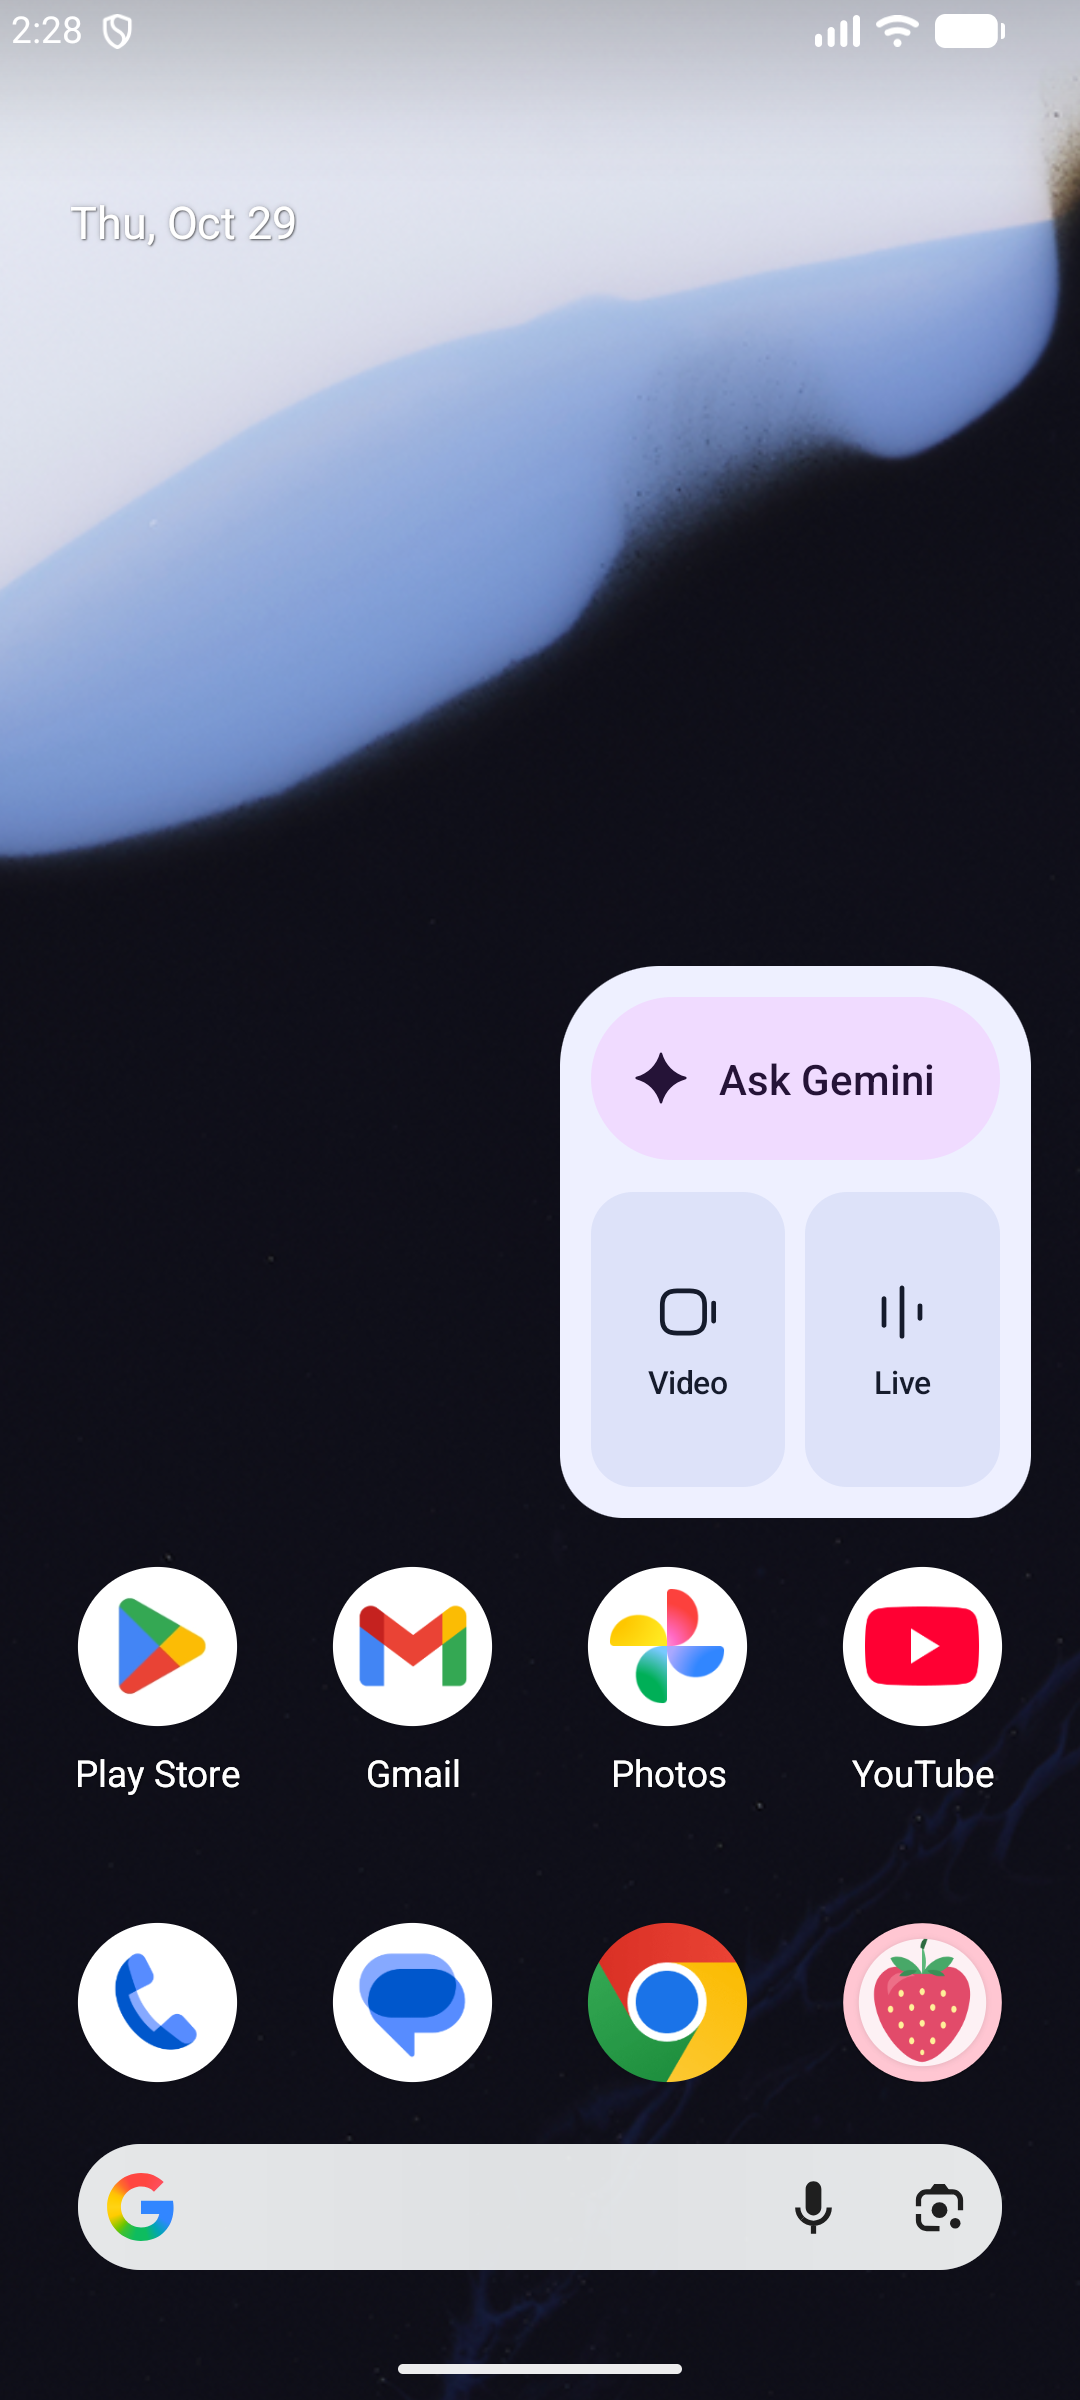
\includegraphics[width=0.48\textwidth]{images/screen_recipe_edit.png}
    \caption{Schermata di Modifica Ricetta: dati generali, selettore categoria con Panini, resa, modificatore cottura e assistente AI.}
    \label{fig:edit}
\end{figure}

\subsection{Dati Generali e Modificatore Peso in Cottura}
Nella prima sezione della scheda \`e possibile impostare:
\begin{itemize}[leftmargin=*]
    \item \textbf{Nome della Ricetta:} Titolo formale della preparazione.
    \item \textbf{Categoria e Tag:} Selezione rapida tra i tag ufficiali (compreso \textit{Panini}) o inserimento di una categoria personalizzata.
    \item \textbf{Resa Base e Unit\`a di Resa:} La quantit\`a di riferimento (es. \textit{4 porzioni}, \textit{1 torta}, \textit{2 bicchieri}, \textit{6 panini}).
    \item \textbf{Modificatore Peso in Cottura (\%):} Campo fondamentale introdotto in SIMO 2.0. Permette di registrare la percentuale di variazione della massa durante il trattamento termico:
    \begin{itemize}[noitemsep]
        \item \textbf{Valori Negativi (Calo Peso):} Es. \texttt{-10\%} per torte e crostate, \texttt{-15\%} per arrosti o \texttt{-8\%} per creme da pasticceria che perdono acqua per evaporazione in forno o sul fornello.
        \item \textbf{Valori Positivi (Resa/Aumento di Massa):} Es. \texttt{+120\%} per pasta secca o riso che assorbono liquidi durante la bollitura raddoppiando o triplicando il proprio peso iniziale.
        \item \textbf{Valore Neutro (0\%):} Per preparazioni a crudo, cocktail o piatti freddi senza variazione ponderale.
    \end{itemize}
\end{itemize}

\subsection{Inserimento e Gestione dei 6 Valori Nutrizionali}
Toccando ciascun ingrediente (Figura~\ref{fig:edit}), si accede alla configurazione analitica dettagliata:
\begin{simobox}{Dati Nutrizionali per 100\,g di Materia Prima}
Oltre al nome, alla dose, al costo commerciale e ai 14 allergeni, per ogni ingrediente \`e possibile registrare i \textbf{6 parametri nutrizionali ufficiali per 100\,g}:
\begin{enumerate}[leftmargin=*,noitemsep]
    \item \textbf{Calorie (kcal):} Valore energetico espresso in chilocalorie.
    \item \textbf{Carboidrati (g):} Contenuto di glucidi per 100\,g.
    \item \textbf{Grassi (g):} Contenuto lipidico per 100\,g.
    \item \textbf{Proteine (g):} Quota proteica per 100\,g.
    \item \textbf{Acqua / Umidit\`a Residua (g):} Grammi d'acqua presenti in 100\,g di prodotto.
    \item \textbf{Sodio (mg):} Milligrammi di sodio (da cui SIMO calcola automaticamente l'equivalente in sale: $\text{Sale} = \text{Sodio [g]} \times 2.5$).
\end{enumerate}
\end{simobox}

\subsection{Banner Assistente AI: Calcola Nutrizione vs Completa Dosi}
Nella parte superiore dell'editor \`e collocato il banner dell'Assistente AI. Toccando \textbf{Apri Assistente AI} si apre la finestra di dialogo operativa (Figura~\ref{fig:ai_options}):
\begin{itemize}[leftmargin=*]
    \item \textbf{Calcola Valori Nutrizionali:} Analizza gli ingredienti gi\`a presenti e calcola esclusivamente i 6 valori nutrizionali per 100\,g basandosi su tabelle ufficiali (CREA / USDA). \textbf{Non modifica n\'e cancella} le pesature, i costi unitari e gli allergeni precedentemente inseriti!
    \item \textbf{Completa Dosi Mancanti:} Perfeziona la ricetta bilanciando grammature, costi, allergeni e valori nutrizionali per gli ingredienti privi di dose, senza aggiungere o rimuovere ingredienti.
    \item \textbf{Genera Ricetta Completa:} Genera da zero l'intera ricetta (dosi, costi, allergeni, valori nutrizionali, calo peso e passaggi numerati).
\end{itemize}

\begin{figure}[h!]
    \centering
    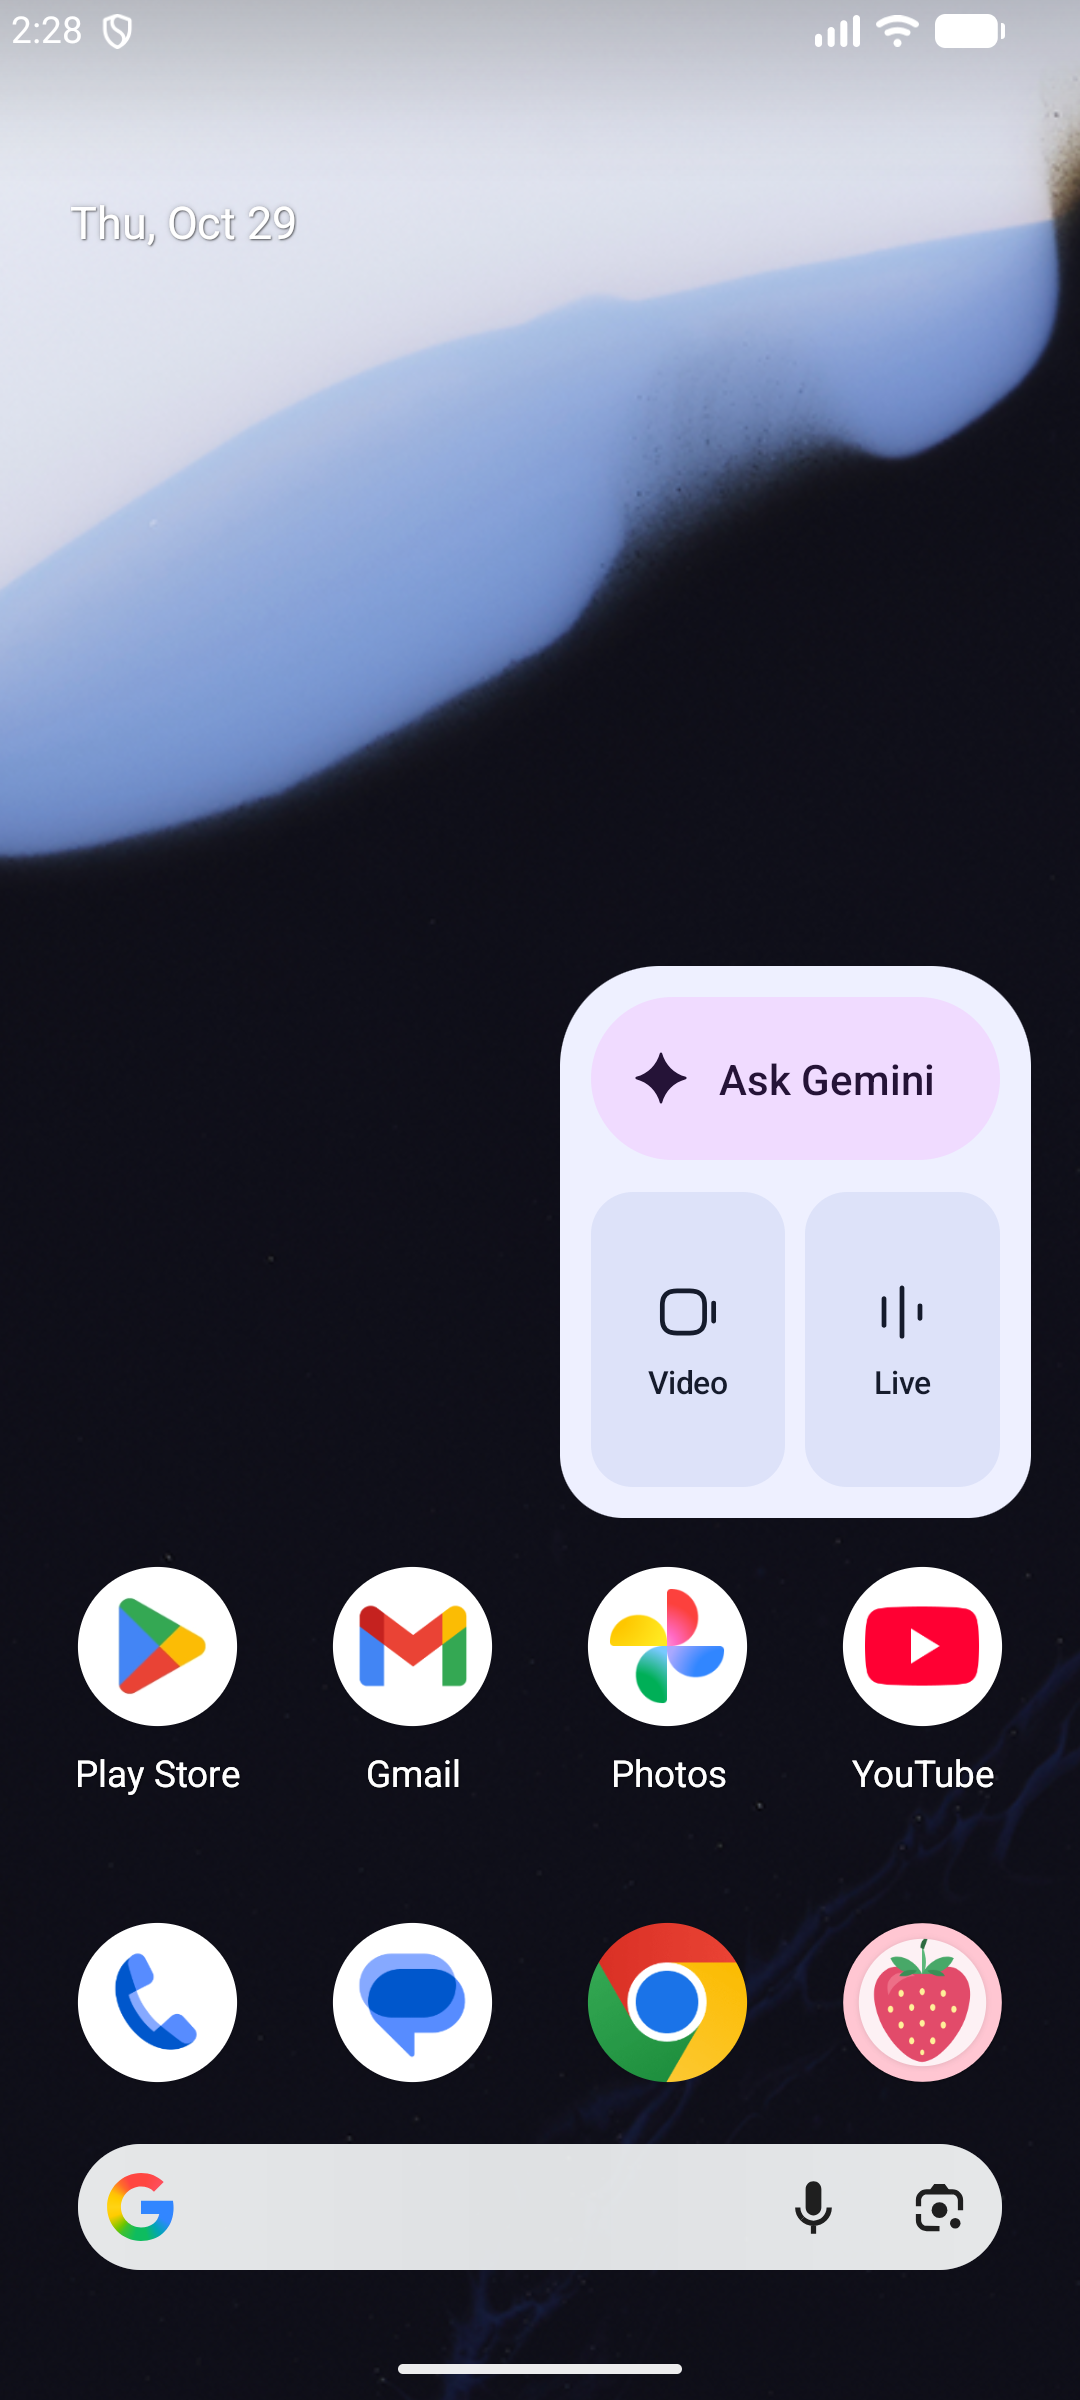
\includegraphics[width=0.44\textwidth]{images/screen_ai_options_dialog.png}
    \caption{Opzioni dedicate dell'Assistente AI nella schermata di composizione ricetta.}
    \label{fig:ai_options}
\end{figure}

\newpage

% ==============================================================================
% SEZIONE 4: RICALCOLO DINAMICO, SCALING E REVERSE SCALING
% ==============================================================================
\section{Il Cuore di SIMO: Scaling, Cottura e Reverse Scaling}

Nel dettaglio di ogni ricetta (Figura~\ref{fig:detail}) risiede il cruscotto di calcolo proporzionale in tempo reale.

\begin{figure}[h!]
    \centering
    
\includegraphics[width=0.48\textwidth]{images/screen_crema_detail_open.png}
    \caption{Schermata Dettaglio: controller di scaling, box Calo Peso in Cottura (crudo vs cotto) e food cost live.}
    \label{fig:detail}
\end{figure}

\subsection{Controller di Resa e Variazione Peso in Cottura}
Il pannello \textbf{Ricalcolo Dinamico} unifica la scalatura delle porzioni con la fisica della cottura:
\begin{itemize}[leftmargin=*]
    \item I pulsanti \textbf{[$-$]} e \textbf{[$+$]} consentono di variare la resa con visualizzazione del moltiplicatore scalare (es. \textbf{1.00x}, \textbf{2.50x}).
    \item \textbf{Confronto Crudo vs Cotto:} Il box mostra sia il peso totale dell'impasto crudo sommato prima della lavorazione (es. \textit{Impasto crudo: 618\,g}), sia il peso del prodotto finito dopo la cottura (es. \textit{Cotto finito: 568.56\,g} con calo dell'8\%).
    \item \textbf{Resa Cotta a Porzione:} SIMO indica il peso netto stimato di ciascuna singola porzione cotta finita (es. \textit{\textasciitilde 71\,g a porzione}).
\end{itemize}

\subsection{Reverse Scaling dalla Dispensa}
Se disponi di una quantit\`a limitata di una materia prima (ad esempio 120\,g di burro anzich\'e 175\,g):
\begin{enumerate}[leftmargin=*]
    \item Tocca la pillola con la quantit\`a dell'ingrediente vincolante;
    \item Inserisci la quantit\`a effettivamente disponibile e conferma;
    \item L'intero albero di componenti e la resa totale si riparametreranno all'istante attorno a quel vincolo.
\end{enumerate}

\newpage

% ==============================================================================
% SEZIONE 5: TABELLA NUTRIZIONALE UE, ALLERGENI E FOOD COST
% ==============================================================================
\section{Dichiarazione Nutrizionale UE, Allergeni e Food Cost}

\subsection{Scheda Nutrizionale Grafica UE (Regolamento UE 1169/2011)}
In fondo alla schermata di dettaglio, sotto la lista degli ingredienti e degli allergeni, compare la nuova \textbf{Dichiarazione Nutrizionale Grafica UE} (Figura~\ref{fig:nutrition_card}):

\begin{figure}[h!]
    \centering
    
\includegraphics[width=0.48\textwidth]{images/screen_nutrition_card.png}
    \caption{Scheda Dichiarazione Nutrizionale UE: valori medi per 100\,g e per porzione, con dicitura di stima e nota cottura.}
    \label{fig:nutrition_card}
\end{figure}

\begin{simobox}{Caratteristiche della Scheda Nutrizionale}
\begin{itemize}[leftmargin=*,noitemsep]
    \item \textbf{Dicitura Ufficiale di Stima:} L'intestazione riporta chiaramente la dicitura \textit{``DICHIARAZIONE NUTRIZIONALE (Stima \textendash{} Reg. UE n. 1169/2011)''}.
    \item \textbf{Doppia Colonna di Riferimento:} I valori medi sono suddivisi su due colonne: \textbf{Per 100\,g} e \textbf{Per Porzione} (con peso esatto della porzione cotta finita).
    \item \textbf{Protezione Tipografica Monoriga per l'Energia:} La riga dell'energia riporta congiuntamente i valori in \textbf{kJ} e in \textbf{kcal} (es. \textit{984 kJ / 235 kcal}) formattati per non andare mai a capo o subire troncamenti.
    \item \textbf{I 7 Parametri Standard UE:} Energia, Grassi, Carboidrati, Proteine, Sale equivalente (derivato dal Sodio moltiplicato per 2.5), Sodio e Acqua (umidit\`a residua).
    \item \textbf{Concentrazione Nutrienti con Modificatore Cottura:} I valori per 100\,g tengono conto dell'evaporazione d'acqua in cottura: se l'impasto perde il 10\% d'acqua, i macronutrienti nei 100\,g di prodotto finito risulteranno proporzionalmente concentrati, riflettendo la reale chimica alimentare!
\end{itemize}
\end{simobox}

\subsection{Allergeni Normativi UE e Food Cost al Centesimo}
\begin{itemize}[leftmargin=*]
    \item \textbf{14 Allergeni UE:} Evidenziati con chip colorati e badge monoriga protetti (\textit{Allergene \#N}), ereditati ricorsivamente da tutte le sotto-ricette.
    \item \textbf{Food Cost in Tempo Reale:} Calcola il costo totale dell'impasto e il costo a porzione/pezzo con equivalenza culinaria 1:1 per densit\`a unitaria ($1\,\text{g} = 1\,\text{ml}$ e $1\,\text{kg} = 1\,\text{l}$), prevenendo distorsioni di prezzo quando i liquidi (es. latte, caff\`e, panna) vengono dosati in millilitri ma tariffati in litri o chilogrammi.
\end{itemize}

\newpage

% ==============================================================================
% SEZIONE 6: COOKING MODE E TIMER INTELLIGENTI
% ==============================================================================
\section{Cooking Mode e Timer Multipli Integrati}

La \textbf{Cooking Mode} (Figure~\ref{fig:cooking} e~\ref{fig:timer}) trasforma SIMO in un cruscotto operativo da banco per la preparazione attiva.

\begin{figure}[h!]
    \centering
    \begin{minipage}{0.48\textwidth}
        \centering
        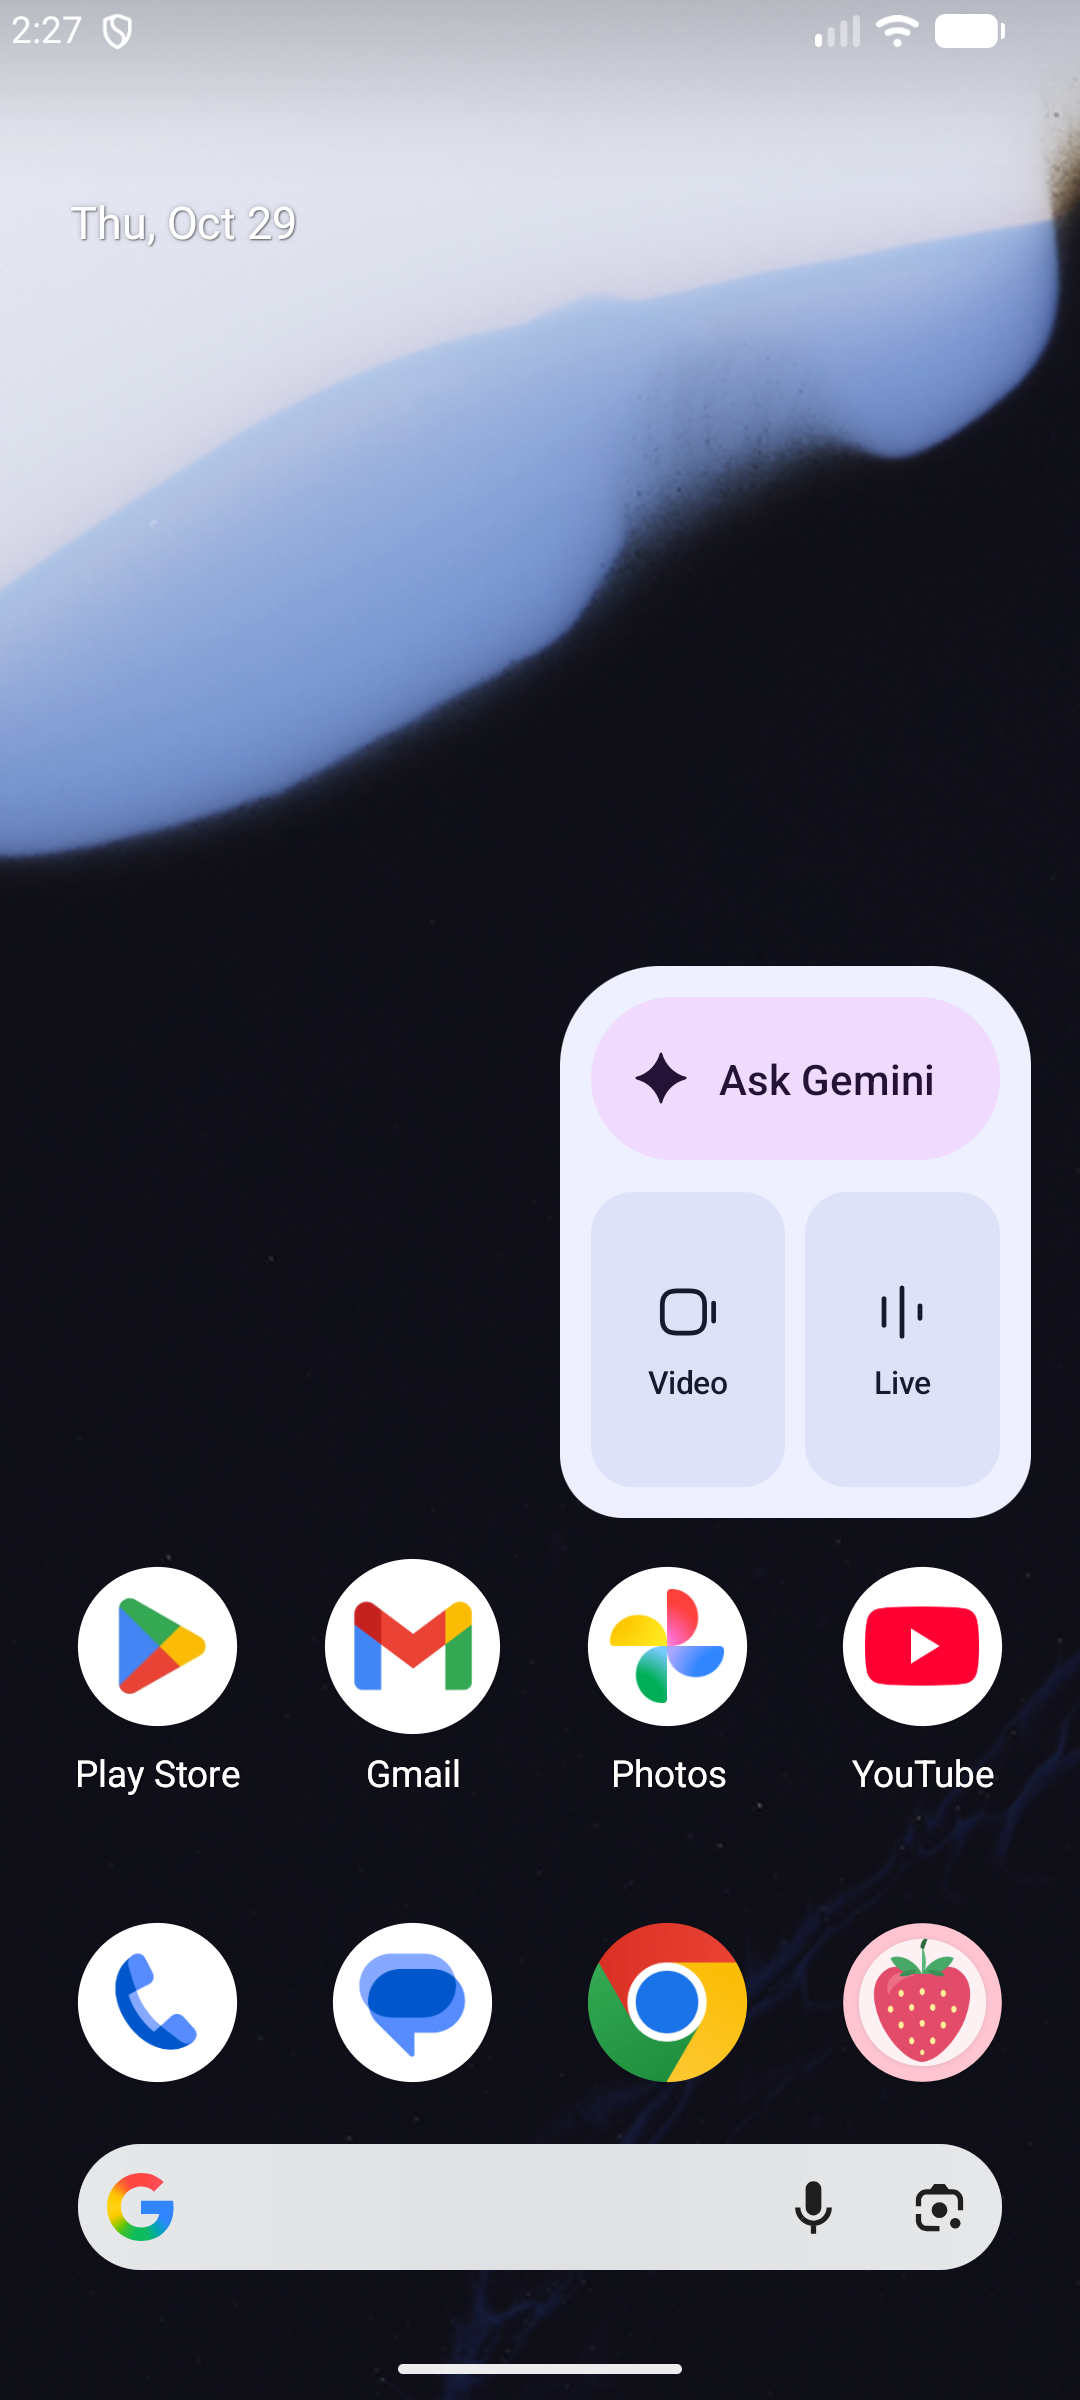
\includegraphics[width=\textwidth]{images/screen_cooking_opened_success.png}
        \caption{Cooking Mode protetta con checklist delle dosi gi\`a scalate.}
        \label{fig:cooking}
    \end{minipage}\hfill
    \begin{minipage}{0.48\textwidth}
        \centering
        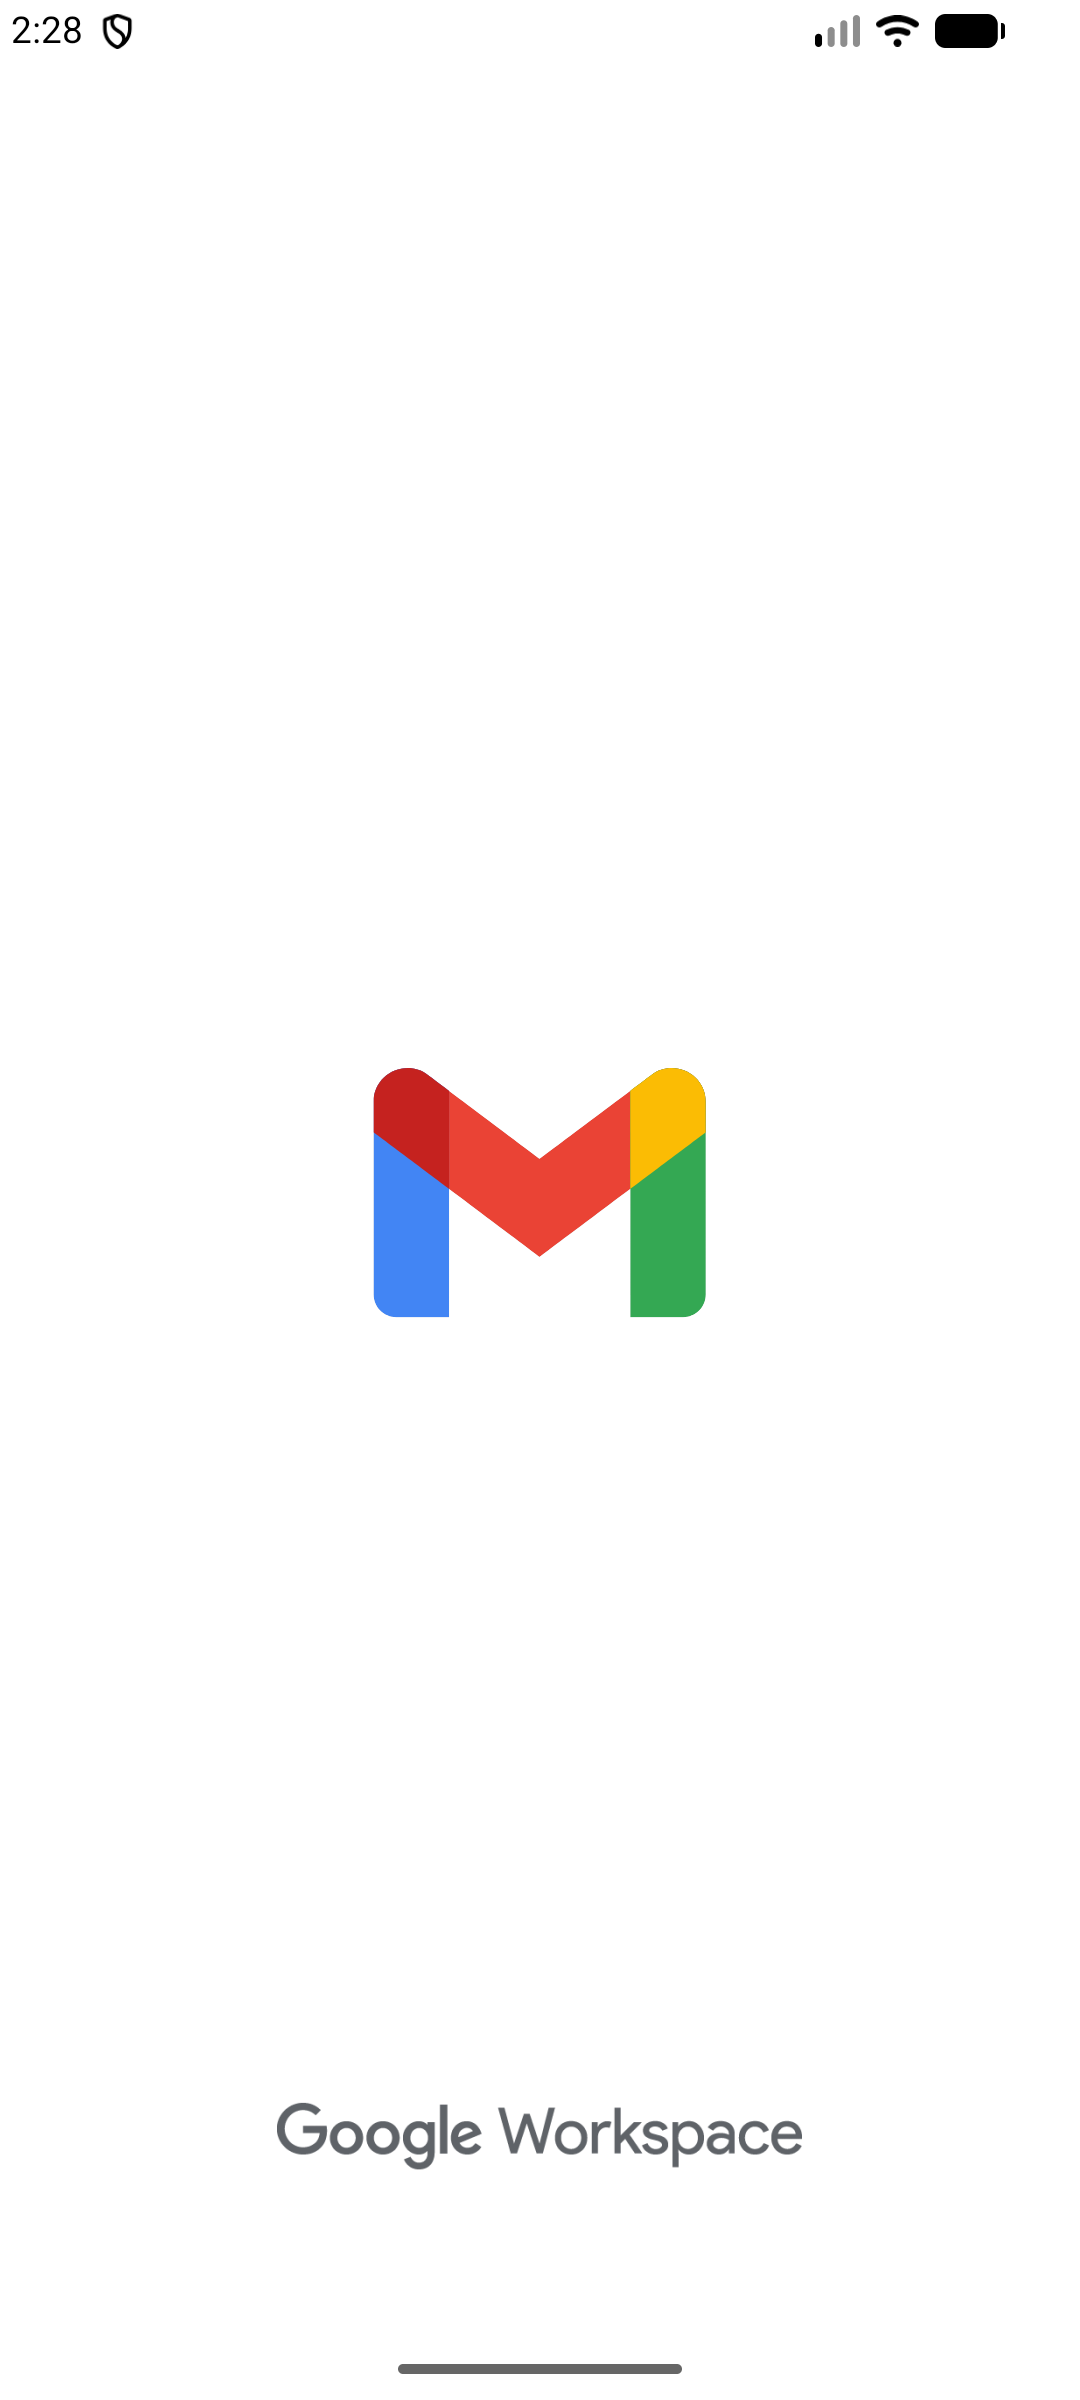
\includegraphics[width=\textwidth]{images/screen_timer_dialog_new.png}
        \caption{Popup Rapido Timer (+30s, +1m, +5m, +10m).}
        \label{fig:timer}
    \end{minipage}
\end{figure}

\begin{itemize}[leftmargin=*]
    \item \textbf{Schermo Sempre Attivo (\textit{Keep Screen On}):} Nessun blackout del display mentre le mani sono sporche o bagnate.
    \item \textbf{Checklist di Pesatura e Passaggi:} Caselle di spunta rapide per segnare gli ingredienti pesati e le fasi procedurali completate.
    \item \textbf{Riconoscimento Automatico dei Timer nel Testo (Figura~\ref{fig:timers_inst}):} Frasi come \textit{``infornare per 35 minuti''} o \textit{``cuocere per 12 minuti''} generano pulsanti interattivi immediati con il conto alla rovescia preimpostato.
    \item \textbf{Resilienza in Background con Foreground Service:} Puoi cambiare app (es. guardare un tutorial su YouTube o rispondere al telefono): i timer continuano a scorrere e suoneranno con allarme acustico e vibrazione allo scadere.
\end{itemize}

\begin{figure}[h!]
    \centering
    
\includegraphics[width=0.48\textwidth]{images/screen_instructions_timers.png}
    \caption{Istruzioni con bottoni timer generati automaticamente dal testo.}
    \label{fig:timers_inst}
\end{figure}

\newpage

% ==============================================================================
% SEZIONE 7: LISTA DELLA SPESA INTELLIGENTE
% ==============================================================================
\section{Lista della Spesa Intelligente}

Accessibile dal menu superiore o direttamente dal dettaglio ricetta tramite il tasto verde \textbf{Aggiungi a Spesa} (Figura~\ref{fig:shopping}):

\begin{figure}[h!]
    \centering
    
\includegraphics[width=0.48\textwidth]{images/shopping_list_verified.png}
    \caption{Lista della spesa intelligente: aggregazione automatica delle dosi e stima economica complessiva.}
    \label{fig:shopping}
\end{figure}

\begin{itemize}[leftmargin=*]
    \item \textbf{Aggregazione Automatica:} Se pi\`u ricette utilizzano lo stesso ingrediente con la stessa unit\`a, le quantit\`a vengono unificate in una sola riga (es. $200\,\text{g} + 150\,\text{g} = 350\,\text{g}$ di burro).
    \item \textbf{Stima del Costo Totale della Spesa:} Calcola in tempo reale la spesa economica complessiva convertendo automaticamente i prezzi registrati al chilogrammo o al litro.
    \item \textbf{Gestione Articoli ``q.b.'':} Gli articoli a dose libera adottano un quantitativo d'acquisto standard (100\,g o 1 unit\`a) per agevolare l'approvvigionamento al supermercato.
\end{itemize}

\newpage

% ==============================================================================
% SEZIONE 8: ASSISTENTE AI BIVALENTE, PDF MULTIPAGINA E BACKUP
% ==============================================================================
\section{Assistente Chef AI, Stampa PDF Multipagina e Backup}

\subsection{Assistente Chef AI Bivalente (Gemini \& ChatGPT)}
SIMO 2.0 integra nativamente due motori di intelligenza artificiale di livello mondiale: \textbf{Google Gemini} e \textbf{OpenAI ChatGPT} (Figura~\ref{fig:ai_dialog}).

\begin{figure}[h!]
    \centering
    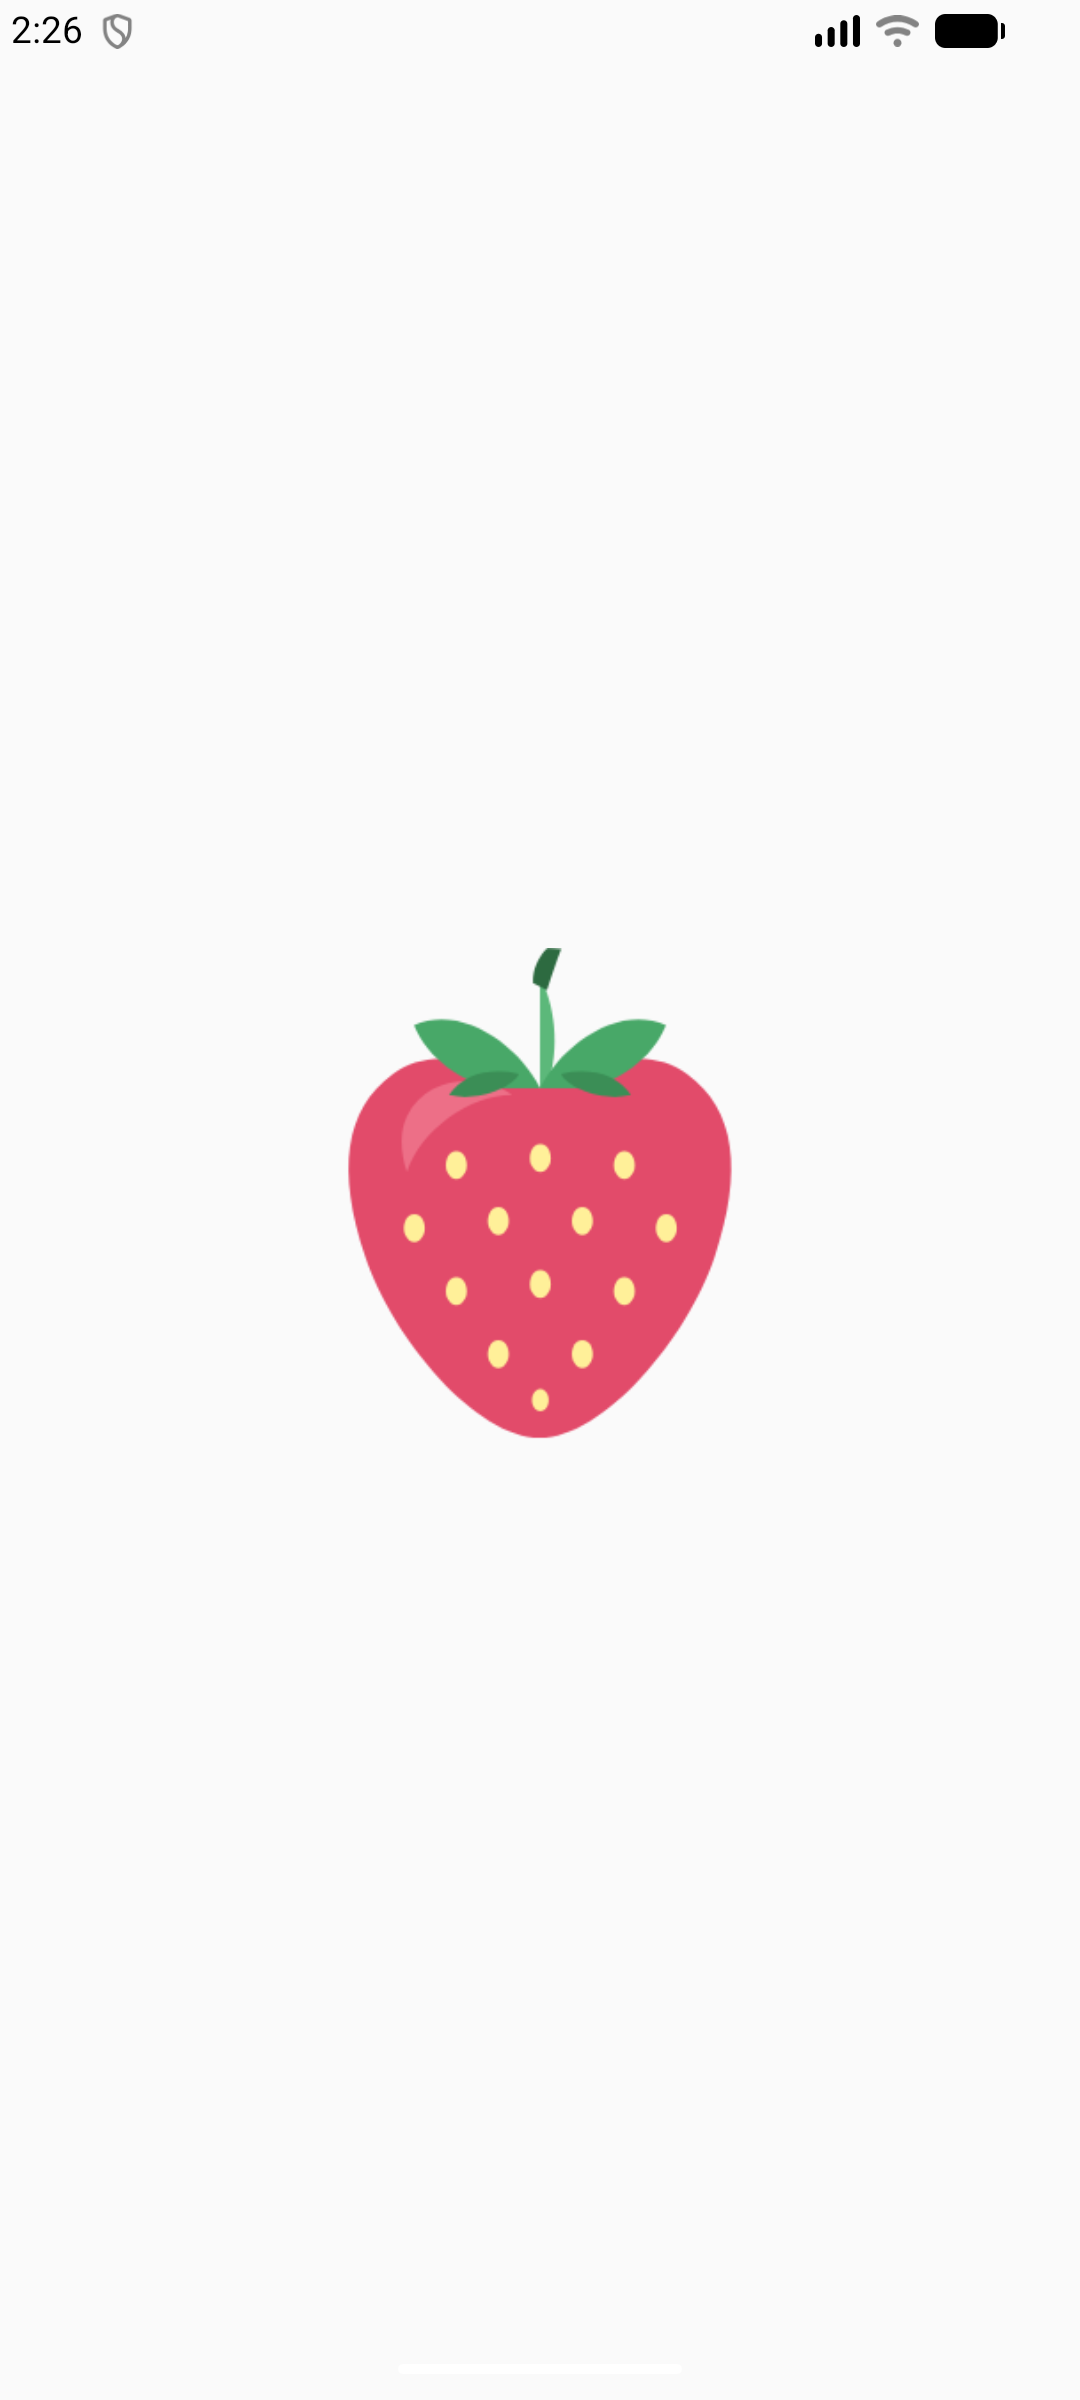
\includegraphics[width=0.48\textwidth]{images/screen_gemini_assistant_dialog.png}
    \caption{Finestra dell'Assistente AI: scelta del provider, prompt guidati e sicurezza hardware KeyStore.}
    \label{fig:ai_dialog}
\end{figure}

\begin{itemize}[leftmargin=*]
    \item \textbf{Preservazione Intelligente dell'Unit\`a di Resa:} Quando imposti un'unit\`a personalizzata (es. \textit{torta}, \textit{bicchieri}, \textit{panini}, \textit{fette}, \textit{crostate}), l'AI valuta la coerenza culinaria con la ricetta richiesta:
    \begin{itemize}[noitemsep]
        \item Se l'unit\`a \`e congruente (es. \textit{torta} per una cheesecake, \textit{bicchieri} per un cocktail o un frapp\`e, \textit{panini} per burger o panini), l'AI \textbf{mantiene la tua unit\`a} e calibra le dosi su di essa!
        \item Solo se l'unit\`a \`e palesemente priva di senso gastronomico (es. \textit{bicchieri} per una pizza o un risotto), l'AI torna a \textit{porzioni}.
    \end{itemize}
    \item \textbf{Valori Realistici e Bilanciati:} I prompt di sistema impongono il massimo rigore gastronomico, dosaggi calibrati, prezzi di mercato italiani e valori nutrizionali fedeli.
    \item \textbf{Sicurezza Hardware-Backed AES-256 GCM:} Le tue chiavi API di Google ed OpenAI sono crittografate nel chip hardware sicuro (\textit{Android KeyStore}) del dispositivo e non vengono mai esportate nei backup.
\end{itemize}

\subsection{Esportazione PDF Professionale A4 (Minimo 2 Pagine)}
Dalla scheda di dettaglio, toccando l'icona \textbf{PDF}, SIMO genera un documento A4 stampabile:
\begin{itemize}[leftmargin=*]
    \item \textbf{Minimo 2 Pagine Garantito:}
    \begin{itemize}[noitemsep]
        \item \textbf{Pagina 1:} Intestazione SIMO, data, resa e porzioni, tabella delle materie prime scalate, box Food Cost, tabella degli allergeni UE e la dichiarazione nutrizionale UE completa;
        \item \textbf{Pagina 2 (e successive):} Interamente dedicata al \textbf{Procedimento di Preparazione}, stampato con testo in nero pieno nitido ad alto contrasto per la massima leggibilit\`a sul banco di lavoro.
    \end{itemize}
    \item Condivisione immediata tramite WhatsApp, Telegram, email, Google Drive o stampa diretta Wi-Fi.
\end{itemize}

\subsection{Backup e Ripristino JSON con Risoluzione Conflitti}
Dalla barra principale puoi esportare l'intero archivio in un file standard \texttt{.json} (schema versione 2) contenente tutti i valori nutrizionali, i costi e i modificatori di cottura. Al momento del ripristino su un nuovo telefono, SIMO ti consentir\`a di risolvere individualmente ogni eventuale conflitto tra ricette nuove ed esistenti.

\end{document}
